\documentclass[runningheads]{llncs}
\usepackage{graphicx}
\usepackage{lipsum}
\usepackage{amsmath}

\begin{document}

\chapter{[Chapter 4] Evaluation}


Evaluation of physics engines in general can be quite challenging, 
especially for quantitative analysis.
Little work has been done in this area as of now, 
likely due to the complexity, systematic bias, and the lack of needs.

The evaluation of this project is split into three parts: Benchmark selection, Quantitative evaluations, and Success criteria.

\section{Benchmark selection}

Quantitative evaluations will be largely comparison-based. 
I will be choosing two open-source physics engines that support similar features to compare against.
The following engines have been found as possible candidates:

\begin{table}[h]
  \centering
  \makebox[\linewidth]{
  \begin{tabular}
  {|c|c|}
  \hline 
  Physics engine                                & Website                                                         \\
  \hline 
  Advanced Simulation Library                   & asl.org.il                                           \\
  Bullet                                        & pybullet.org                                           \\
  Newton Game Dynamics                          & newtondynamics.com/forum/newton.php                      \\
  Open Dynamics Engine                          & www.ode.org                                            \\
  PAL              & www.adrianboeing.com/pal                                \\
  PhysX                                         & www.nvidia.com/en-gb/geforce/technologies/physx        \\
  Project Chrono~                               & projectchrono.org                                      \\
  Siconos                                       & nonsmooth.gricad-pages.univ-grenoble-alpes.fr/siconos  \\
  SOFA & www.sofa-framework.org                                 \\
  Tokamak physics engine                        & github.com/isegal/TokamakPhysics                        \\
  \hline
  \end{tabular}
  }
\end{table}

They have then been further narrowed down in consideration of supportability, documentation and popularity. I end up choosing the following physics engines as benchmarks:

\begin{table}[h]
  \centering
  \makebox[\linewidth]{
  \begin{tabular}
  {|c|c|}
  \hline 
  Physics engine                                & Reason???TBA, +screenshots, +brief description on setups                                                         \\
  \hline 
  PhysX                                         & www.nvidia.com/en-gb/geforce/technologies/physx        \\
  SOFA & www.sofa-framework.org                                 \\
  \hline
  \end{tabular}
  }
\end{table}


\section{Quantitative evaluations}

The functionalities of selected physics engines along with mine will be evaluated through a series of small runtime tests.
The tests partially drew inspiration from other existing researches on physics engines\cite{seugling2006evaluation}.

\subsection{Bounce test}

\subsubsection{Setup}

To test whether the engines could handle object collisions, I measure if the momentum and energy are preserved.

Two identical cubes will be placed in a world with no gravity. 

Cube A, the one on the left, is located at $(0, 0, 0)$, and is moving along the $+$x direction with a velocity of $\SI{1}{\m\per\s}$.

Cube B, the one on the right, is located at $(\SI{5}{\m}, 0, 0)$, and is moving along the $-$x direction with a velocity of $\SI{1}{\m\per\s}$.

Both cubes are 1x1x1 and have a mass of $\SI{1}{\kg}$. The coefficient restitution $\epsilon$ is a variable that ranges between $0$ and $1$.

\begin{center}
  \makebox[\textwidth]{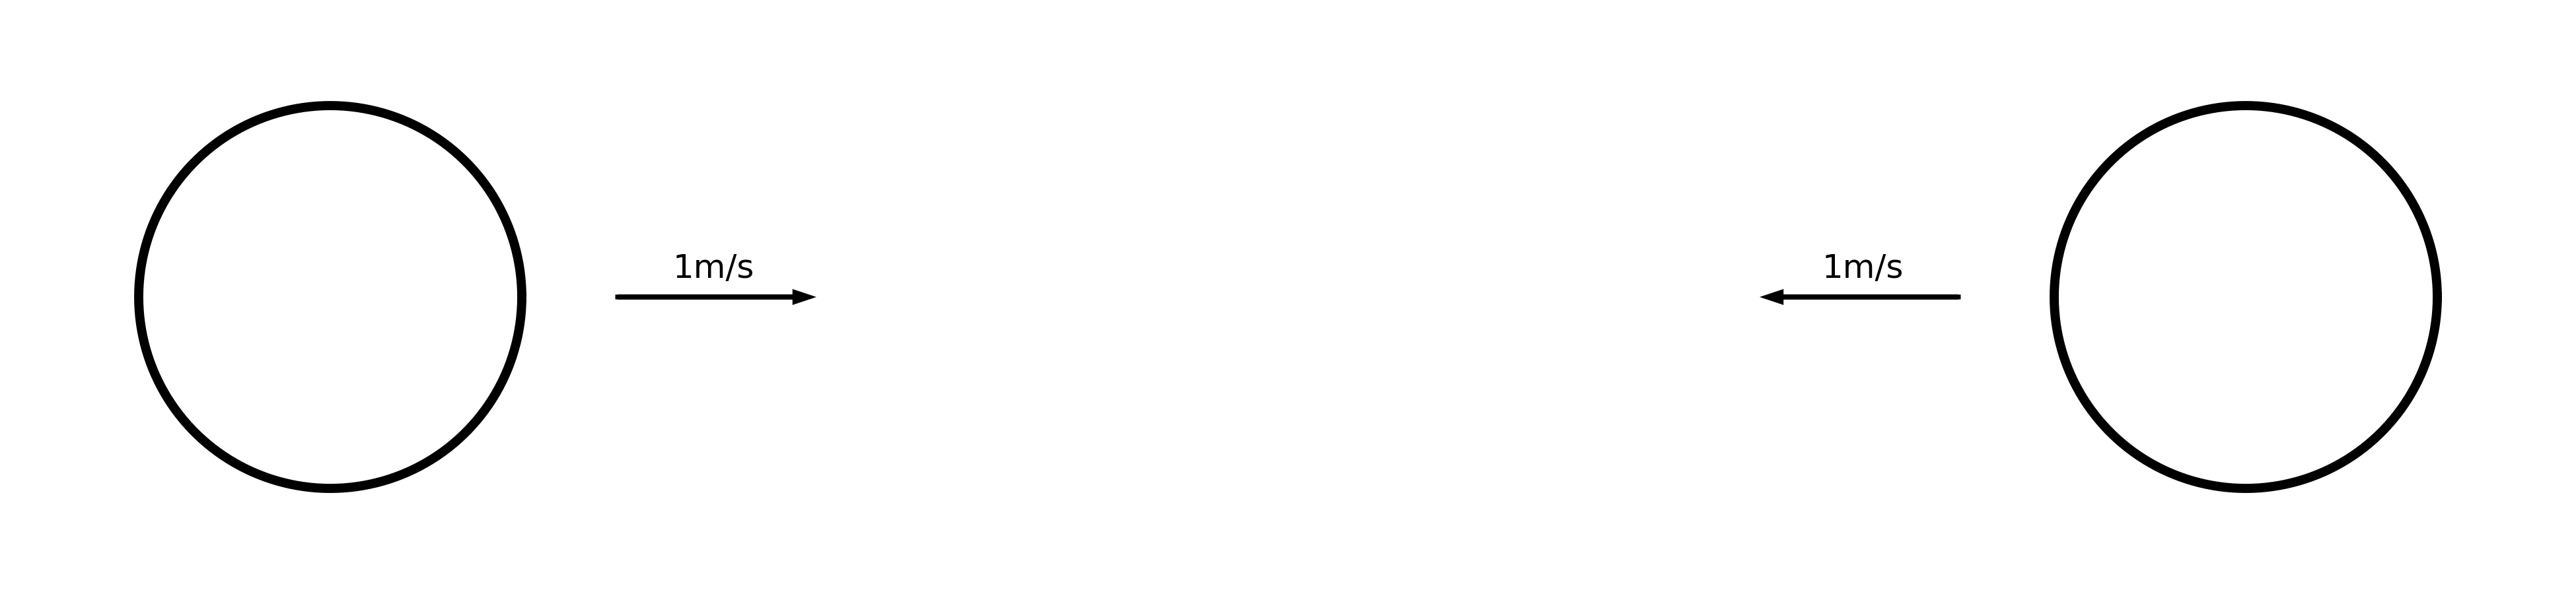
\includegraphics[width=\textwidth]{img1.png}}
\end{center}

Theoretically, the sum of momentum vectors should stay at $(0, 0, 0)$, and the total energy at $\SI{1}{\J}$.
The actual sum of momentum and total energy, as simulated by the engine, will be plotted against time.
The less these values vary, the more accurate the simulation is.

\subsubsection{Result}

All perfectly correct, for all engines. [fig]

As seen in [fig], both the sum of momentum and the total energy stay true to the theoretical results with no noticeable inaccuracies. This is a very basic bouncing task, so as expected all physics engines could reliably accurately simulate it.

\subsection{Support test}

\subsubsection{Setup}

A box will be placed on a fixed inclined plane. The coefficient restitution $\epsilon$ is set to be $0$ - this means a perfectly inelastic collision happens between the box and the plane, so the plane should be able to support the ball. Test if the ball could slide down the plane in an accurate manner. In order to simulate the plane being "fixed" while still being a cuboid rigid body, its mass will be set to infinite, and will be carefully placed with some initial rotation.

The plane passes through the origin $(0, 0, 0)$ and is sufficiently long to hold the cube. The experiment is mostly within the $x-z$ plane. The cube is 1x1x1, and its center of mass is placed at $(-20\cos \theta + \frac{1}{2}\sin \theta, 0, 20\sin\theta+\frac{1}{2}\cos \theta)$. This means its middle contact point with the plane is always $d=20$m from the origin. Constant gravity $G = \SI{10}{\N}$ will be applied to the cube. At any none $0$ degree angle $(\theta > 0)$, the cube should slide down the plane. The time it takes for the $x$ coordinate of its centre to reach $\frac{1}{2}\sin \theta$ will be measured and checked with the theoretical result. Then the experiment will be repeated for different angles $\theta$ within the range $(0, \frac{\pi}{2})$.

In order to obtain a theoretically perfect result, consider a cube moving frictionless slope. Its acceleration along the slope should be $a=\frac{G}{m}\sin \theta$. If the time it takes when accelerating from a static position is $t$, the distance travelled should be $\frac{1}{2}at^2$. So the theoretical time it takes to reach the origin should be $t_0=\sqrt{\frac{2d}{a}}=\sqrt{\frac{2dm}{G\sin \theta}}=\frac{2}{\sqrt{\sin\theta}}$.

\begin{center}
  \makebox[\textwidth]{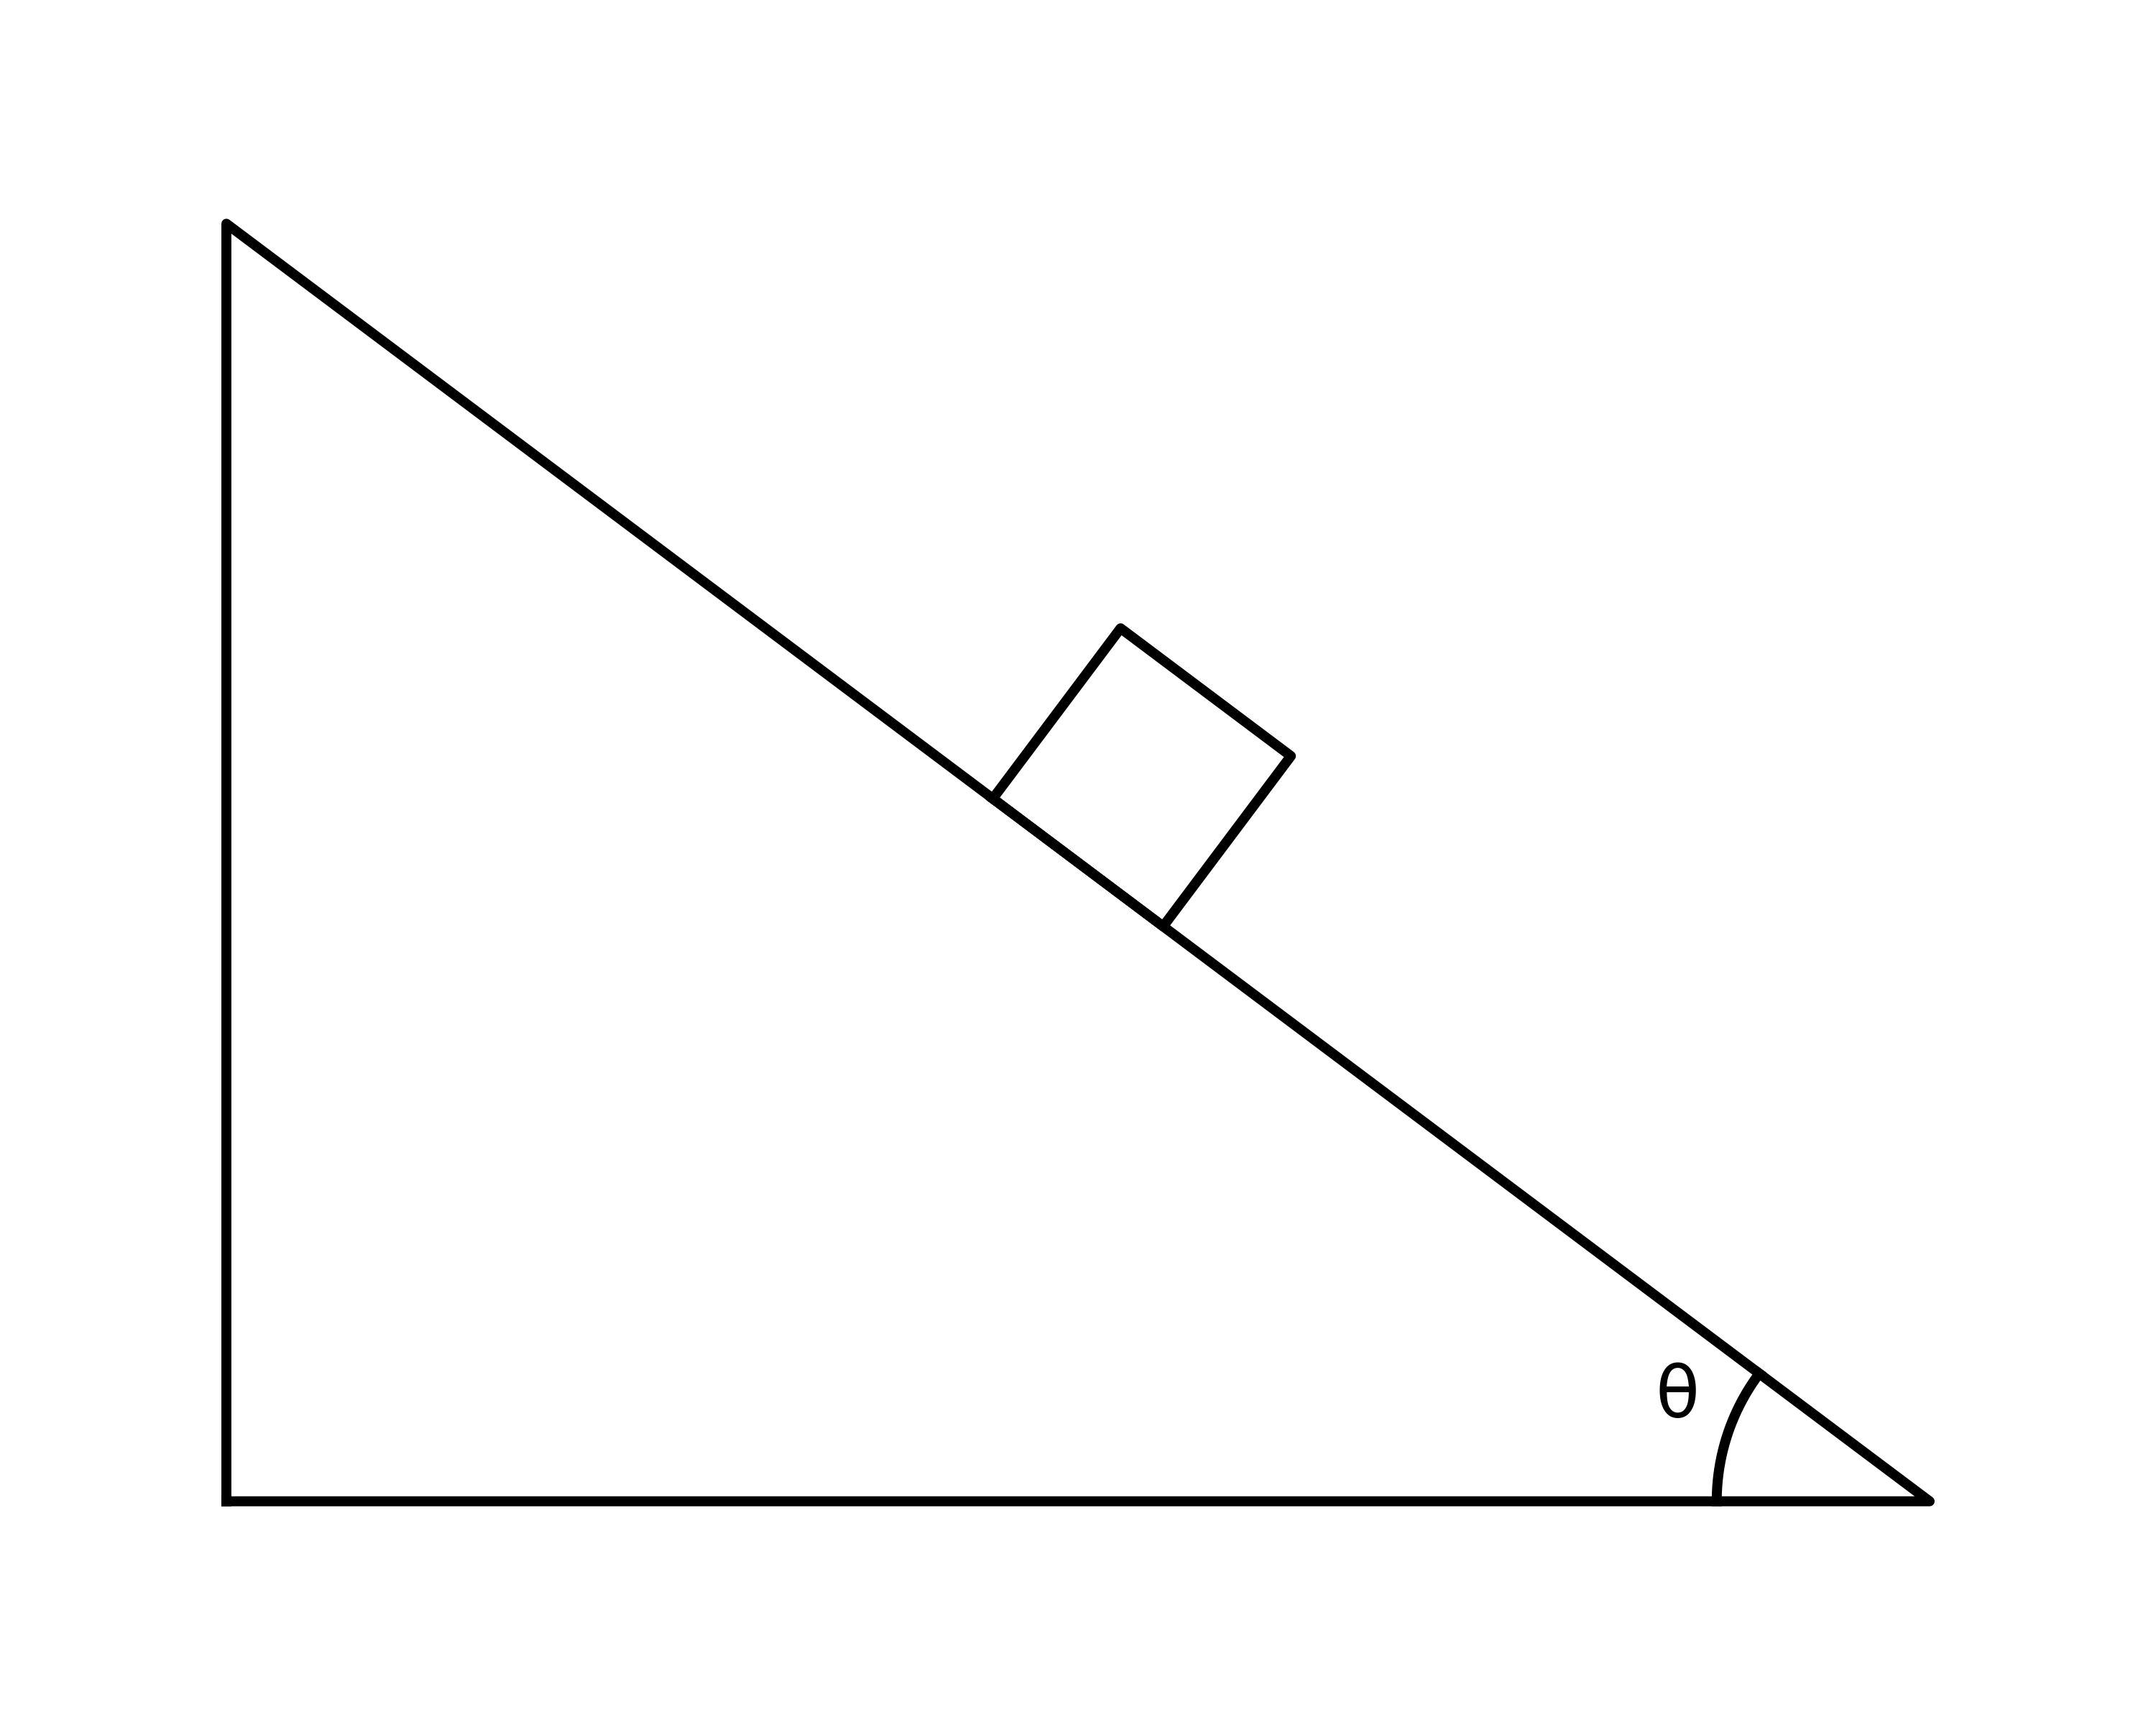
\includegraphics[width=0.5\textwidth]{img2.png}}
\end{center}

\subsubsection{Result}

5, 7.2, 7.433
10, 5.04, 5.167
20, 3.5, 3.633
30, 2.88, 2.900
40, 2.54, 2.567
50, 2.32, 2.333
60, 2.18, 2.233
70, 2.08, 2.133
80, 2.04, 2.100
85, 2.02, 2.067

As seen in [fig], in general the time it takes for the cube to slide down matches with the theoretical result, but in general all the engines give a slightly higher result. This is likely due to accumulated inaccuracies of repeated collisions along the slope. From the view of a physics engine, the cube repeated collides with the slope, and the result is its downwards momentum transfers into sliding momentum. The transfers needed to be calculated every time, so it could be slightly delayed compared to the theoretical analysis.

\subsection{Pendulum test}

\subsubsection{Setup}

Have a pendulum setup like in the following figure.

A small object is attached to a fixed point using a "thread" with a length of $L=\SI{10}{\m}$. To simulate such a "thread" in my physics engine, the object is simply "pulled" back up after unconstrained simulation at each time step.

The initial angle between the bar that connects the sphere and an imaginary vertical line through the fixed point is $\theta$.

\begin{center}
  \makebox[\textwidth]{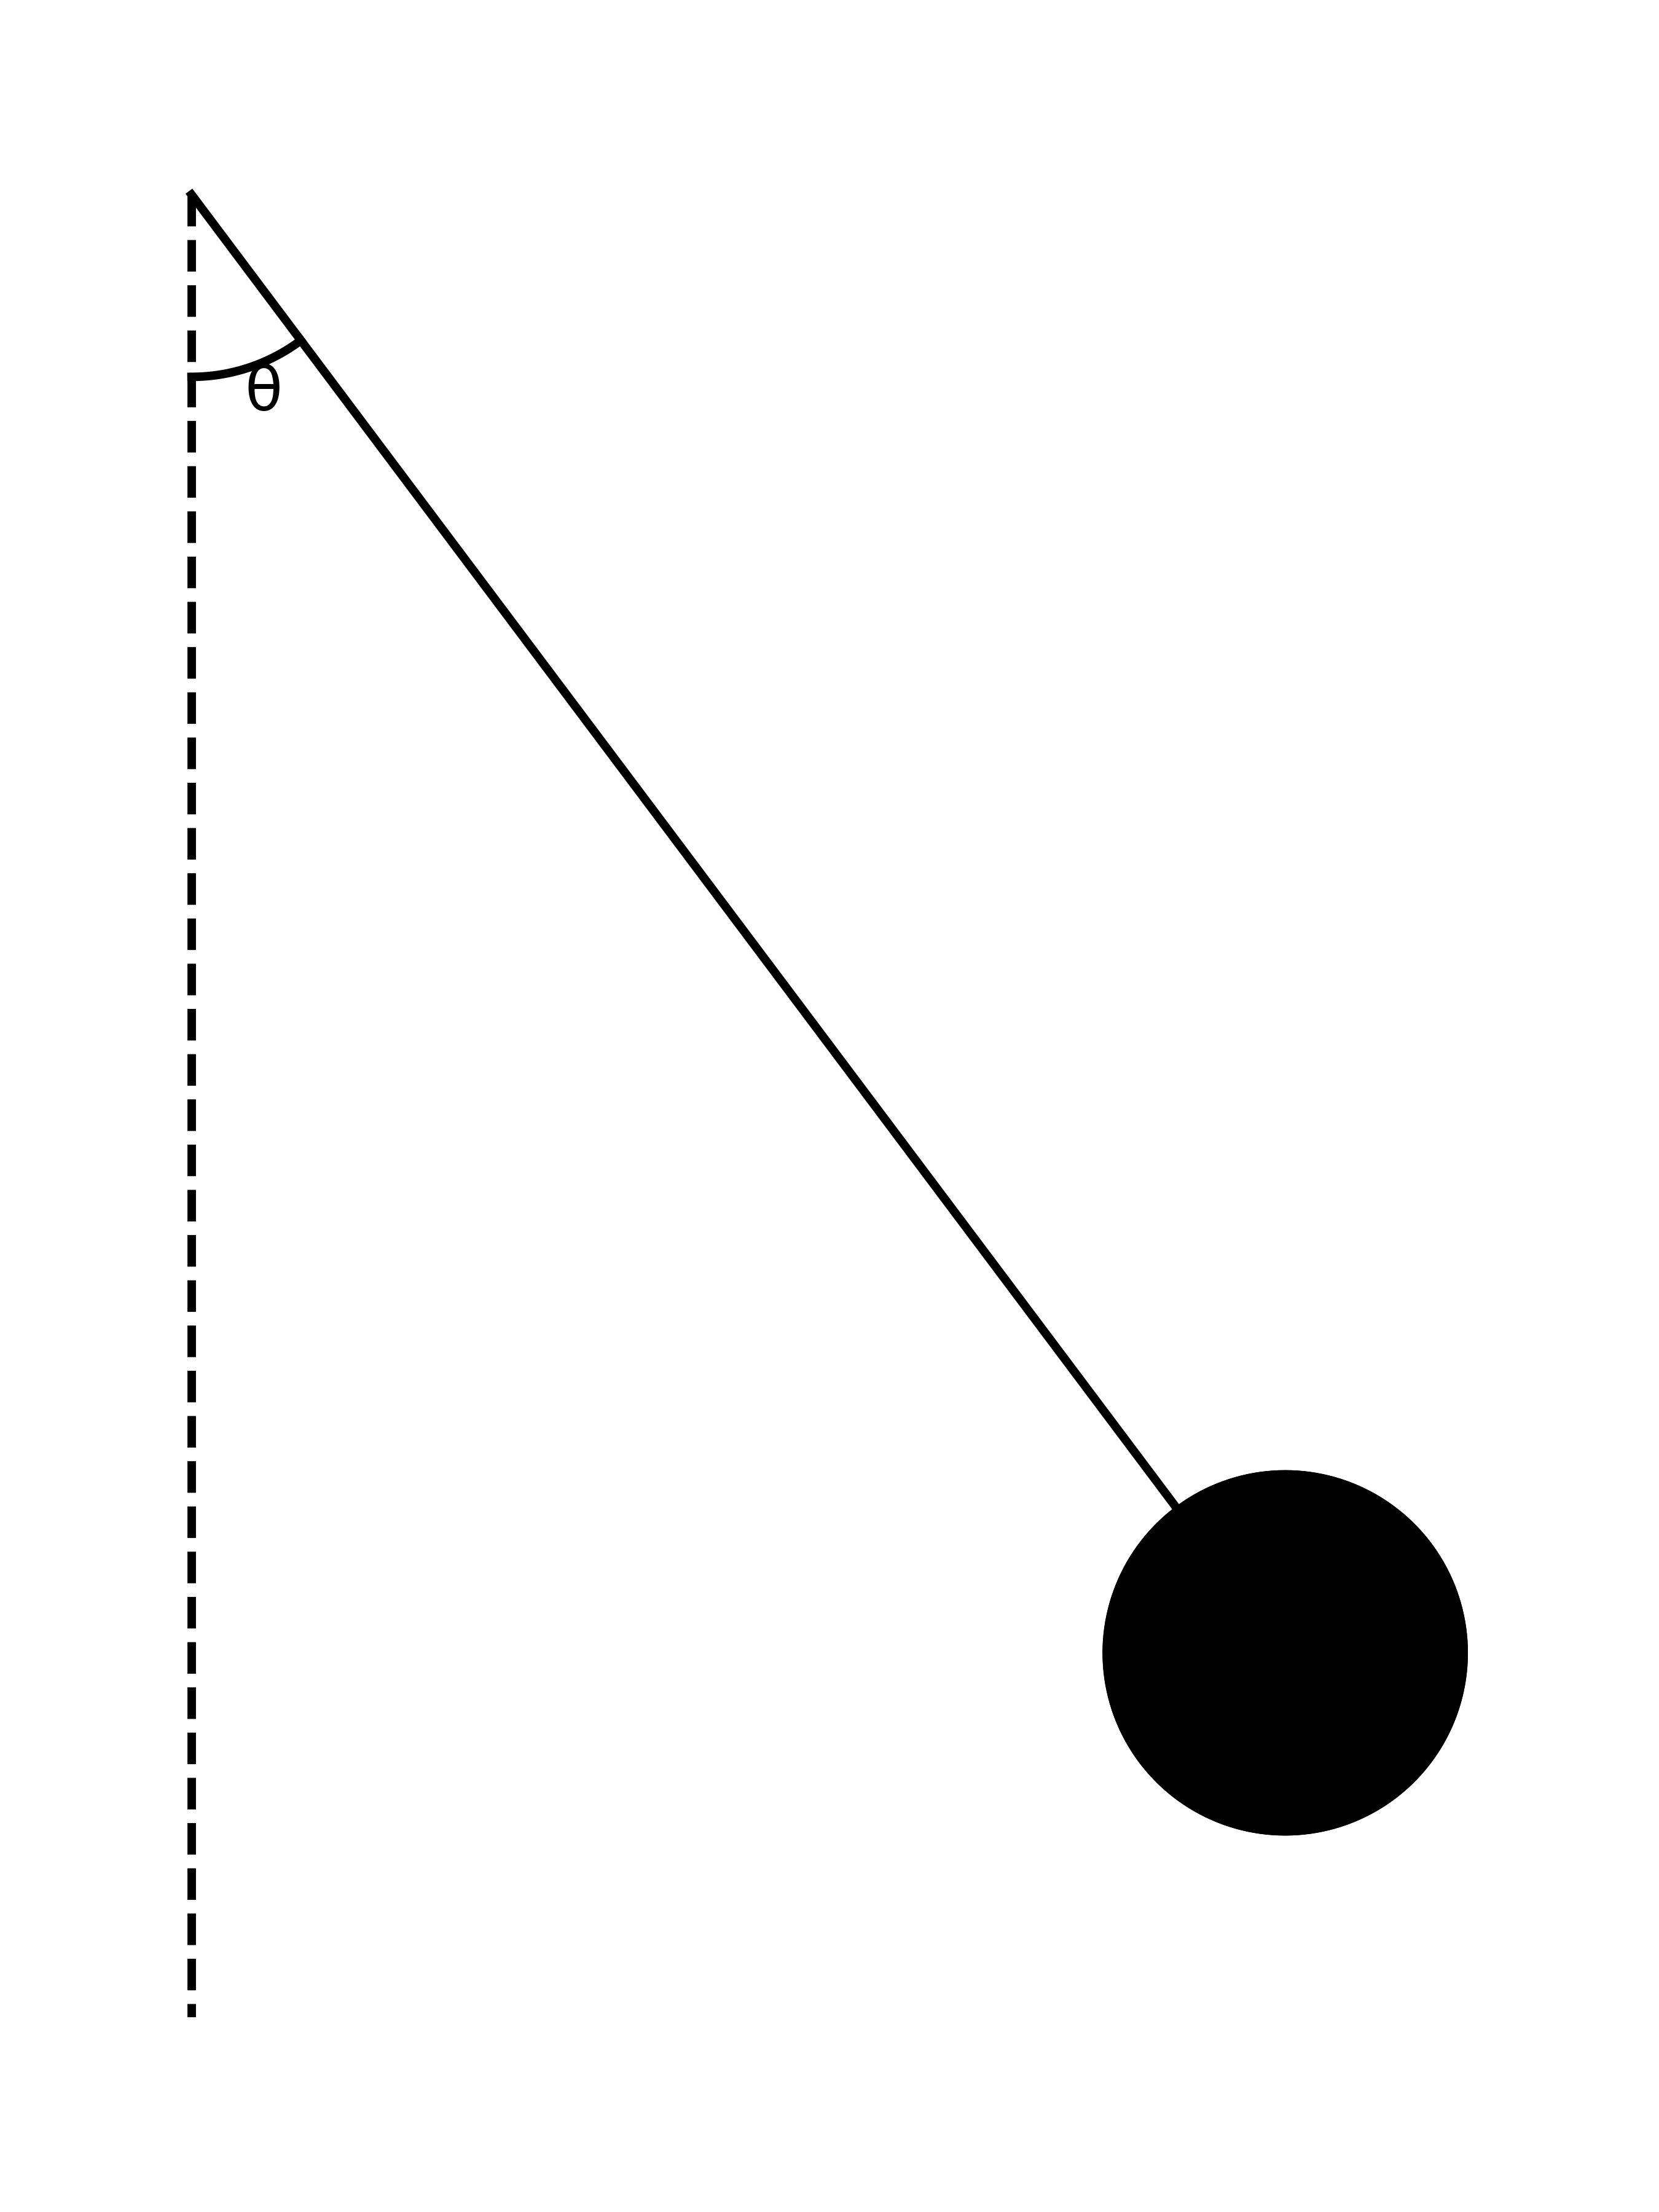
\includegraphics[width=0.3\textwidth]{img3.png}}
\end{center}

$\theta$ is gradually increased from $5\degree$ to $85\degree$.
For each $\theta$, 
the period of the pendulum is measured by recording the time it takes for the sphere to reach its lowest point $5$ times.

Theoretically, the period of a pendulum is

\begin{equation}
T = 2  \pi \cdot \sqrt{\frac{L}{g}}
\end{equation}

The periods as simulated by the engines will be plotted against the angle $\theta$.

\subsubsection{Result}

5, 18.24 (/ 2.5)
10, 18.30
20, 18.26
30, 18.26
40, 18.30
50, 18.36
60, 18.46
70, 18.58
80, 18.80
85, 18.93

As seen in [fig], this is an experiment where all the physics engine deviate quite a bit from the theoretical results. Engines generally take a longer time to swing the pendulum as the degree increase, possibly due to the accumulation of correction errors from the thread constraining the object, which should have resulted in an arc, but got simulated as small segments.

\section{Success criteria}

Success criteria from the project proposal:

\begin{itemize}

\item Implement all basic modules: Object modelling, Collision detection, Bounce, Friction, Stability.

\item Evaluate the engine by comparing it with popular existing engines with simple experiments.

\item Demonstrate that the engine works with screenshots of simple examples.
\end{itemize}

For extensions (ordered by priority):

\begin{itemize}
\item Implement fluid dynamics.

\item Implement different versions of the engine for whether GPU is used, and for other interesting parameters like the number of cores used. 
Then evaluate the performance.

\item Implement real-time rendering, which should allow the project to meet all previous criteria without third-party rendering libraries. 

\item Implement soft-body dynamics.

Referring back to the success criteria, I consider all core criteria to be completed and successful. Extensions were attempted but not as successful. All basic modules related to rigid body simulation are implemented and evaluated with simple experiments. The followings are some example screenshots of the resulting rendered video.

\begin{center}
  \makebox[\textwidth]{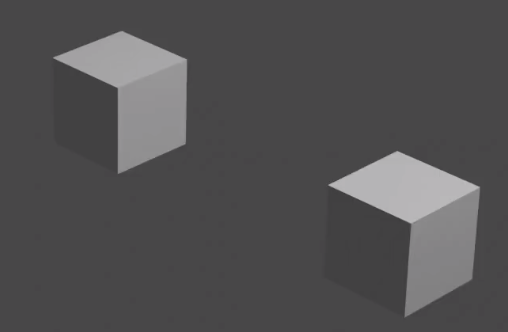
\includegraphics[width=\textwidth]{Untitled.png}}
\end{center}

[fig]

The results of the evaluations also show a high correlation with real-life physics results. Therefore, my physics engine is indeed capable of simulating simple rigid body interactions.

\subsection{Limitations}

As seen from some of the experiments [ref], the inaccuracies of simulating certain interactions are slightly greater than popular existing physics engine. Furthermore, external functionalities, configurable options, API documentations and bug considerations are definitely not as complete as other popular physics engines. Most modern physics engines provide several alternate simulation methods, for example for solving differential equations mentioned in [ref]. Some extensions like liquid simulation are also not in a working state in my engine but is supported by many other engines. On the other hand, they possess dedicated maintenance by large groups of developers, so it is not reasonable to aim at surpassing their massive project in every possible way.

\end{itemize}

\noindent\rule{12cm}{0.4pt}


\end{document}
